\chapter{Sketch It, Make It: Details}

The previous chapter gave an overview of SIMI's architecture. This
included an introduction of SIMI's recognition process.
(Section~\ref{sec:recognition-architecture}). This chapter gives
details on how each recognizer works. 

First, SIMI's corner finding and segmentation strategy is
described. This process is necessary to most recognition, and is what
produces geometric output like lines and arcs. Next, the three types
of recognizers are described: including Dynamic, Pen Up, and Delayed
recognizers. All sketch based interaction techniques are detailed in
these sections.

\section{Ink Parsing}
\label{sec:corner-finder}

Ink parsing is the process of identifying useful characteristics of
raw ink, such as the locations of corners, curvature at specific
points, and the likely identities of segments like lines or curves.

In the following sections, there are two different ways to measure
distance: Euclidean and Curvilinear (see
Figure~\ref{fig:distance-measures}). Euclidean distance is the
measurement most people are familiar with: this is how far apart two
points are on the 2D plane. Curvilinear distance follows the ink
stroke path. In the figure, points A and B are close together in the
Euclidean sense, but are farther apart in the Curvilinear sense. The
Euclidean and Curvilinear midpoints are also depicted in
Figure~\ref{fig:distance-measures}. 

\begin{SCfigure}%[t]
  \centering
  \caption[Euclidean vs. Curvilinear Distance]{Two ways to measure
    distance: Euclidean vs. Curvilinear. The Euclidean distance from A
    to B is direct ($length=18$). Curvilinear distance from A to B
    follows the path indicated ($length=86$). Each measurement
    approach has a related midpoint, indicated as smaller dots.}
  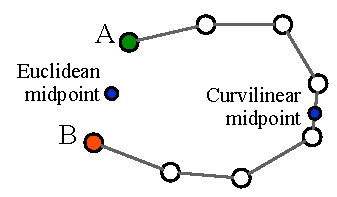
\includegraphics[width=3in]{img/distance-measures.pdf}
  \label{fig:distance-measures}
\end{SCfigure}


SIMI's ink parsing strategy is simpler than many other approches from
the SBIM literature. Others, like the strategies taken by
Sezgin~\cite{sezgin-early-processing} or Wolin~\cite{wolin-smr},
combine both \textit{time} and \textit{curvature} information when
corner finding. SIMI's approach relies only on curvature, but still
achieves good results.

When the user completes a stroke, the ink parser is invoked. First it
assigns a curvature value to each point. Next, a corner finder uses
this data to identify which (if any) points along the stroke are
corners. Last, the system analyzes the regions between corners to
determine the most likely segment type. The output of this process is
the set of segmets formed in the last step. I will detail each of
these steps now.

\subsection{Curvature}

\begin{figure}
  \centering
  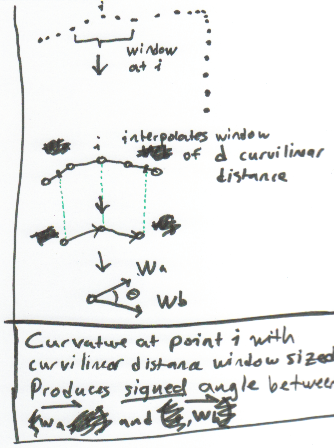
\includegraphics[width=2in]{img/curve-diagram.png}
  \caption[Curvature]{Illustration of how SIMI computes curvature about point $p_i$.}
  \label{fig:curvature-diagram}
\end{figure}


Figure~\ref{fig:curvature-diagram} illustrates how curvature is
calculated. A rough ink stroke has a series of points that are not
evenly spaced out. Sometimes, they may be very close together (for
example, when the user draws slowly). To determine the curvature at an
individual point, we must look at a nearby region called a
\textit{window}, rather than the immediate neighbors. Without this
window, the curvature would be unreliable when points are very close
together.

The window's size $w$ is determined by the current zoom factor. When
the zoom factor is 1 (meaning there is a 1:1 ratio between model and
screen coordinates), the window size is 20 (corresponding to 20
pixels). To calculate the window boundaries at point $p_i$, the corner
finder begins at $p_i$ and traverses the stroke backwards and forwards
by half the window size. It computes interpolated points $w_a$ and
$w_b$ that are exactly $w/2$ units along the stroke to $p_i$. It then
forms two vectors: $v_a$ from $w_a$ to $p_i$, and $v_b$ from $p_i$ to
$w_b$.

The signed curvature $\theta$ for $p_i$ is computed directly from
these two vectors. The magnitude is determined by their dot product;
the sign is determined by the cross product.

\begin{samepage}
\begin{equation}
  \theta_{unsigned} = \arccos \frac{v_a\cdot v_b}{|v_a| |v_b|}
\end{equation}

\begin{equation}
  \theta = \left\{ 
  \begin{array}{r l}
    \theta_{unsigned} & \quad \text{if } |v_a \times v_b| \geq 0\text{,}\\
    -\theta_{unsigned} & \quad \text{otherwise}\\
  \end{array} %\right\}
\end{equation}
\end{samepage}

It is tempting to use $\arctan$ to calculate curvature because it is a
simple calculation. However, this leads to discontinuities when the
vertical change is zero. The approach described above is valid for any
orientation.

\subsection{Isolate Corners}

Now that each point's curvature has been calculated, we can identify
corners. This is a two-step process illustrated
in~Figure~\ref{fig:corner-finding}. First, clusters of high curvature
are identified. To be a member of such a cluster, the absolute value
of a point's curvature must be greater than some threshold. In the
current version of SIMI this value is 45 degrees.

\begin{figure}
  \centering
  \begin{subfigure}[t]{0.4\textwidth}
    \centering
    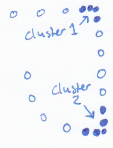
\includegraphics[width=1in]{img/corner-clusters.png}
    \caption{Clusters of high curvature.}
    \label{fig:corner-clusters}
  \end{subfigure}
  \hspace{1cm} % spacing, do what you need
  \begin{subfigure}[t]{0.4\textwidth}
    \centering
    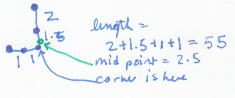
\includegraphics[width=2in]{img/corner-isolation.png}
    \caption{Corner point is closest to middle of cluster.}
    \label{fig:corner-isolation}
  \end{subfigure}
  \caption[Corner finding]{Corner finding involves clustering nearby
    points with high curvature, and choosing the point closest to the
    curvilinear middle of each cluster.}
  \label{fig:corner-finding}
\end{figure}


Once clusters have been computed, a corner is found for each. A
cluster's corner is simply the point closest to the curvilinear
middle. In other words, if the distance along stroke from the
beginning to the end of the cluster is 9, the corner is the point in
the cluster that is nearest to the interpolated point 4.5 units from
the cluster beginning. 

In addition to the corners discoved in this process, the stroke's
first and last points are also included as `corners'. This is for the
convenience of the next step where segments are identified.

\subsection{Identify Segment Types}

The last step in ink parsing is to identify segment
types. Table~\ref{tab:segment-types} in the previous chapter describes
the possible segment types. For each segment type there is a
corresponding segment finder. The segment finders for `open' types
(Line, Arc, Spline) operate on regions between corners. The remaining
segment finders are identified by examining the raw ink directly, and
do not use corner data.

Like semantic sketch recognizers, it is possible for multiple segment
finders to positivly identify ink. To mitigate this, segment finders
operate on a priority system. The priority is: Dot, Circle, Ellipse,
Blob, Line, Arc, and Spline. In other words, if the Dot finder
identifies a dot, there is no possibility of the associated ink being
identified as a Circle.

\subsubsection{Dot Finder}

The dot finder examines the entire ink stroke. If the entire stroke
was made in less than some threshold value (currently 180
milliseconds), it is always considered a dot. Otherwise, it continues
by computing the convex hull of all stroke points. Two properties of
the hull are used next: the area and the aspect ratio. If the ratio
defined by $ratio = area/aspect$ is less than 120, it is a dot. If
not, there is one final check to make. The stroke's point density is
computed. This is the number of points in the original ink stroke,
divided by the hull's area. If $ratio/(0.3 + density)$ is less than
120, it is a dot.

%% The thresholds used in this section (and many others) were determined
%% by trial and error. Some (such as point density) might need to be
%% changed dramatically if different hardware is used. For example, these
%% numbers were found using a default mouse driver, which reports only
%% integer positions. Ink strokes will be less dense than if a proper
%% tablet driver reports floating point locations.

\subsubsection{Circle and Ellipse Finder}

Circles, Ellipses, and (in the next part) Blobs are the three
\textit{closed} segment types. A segment is closed if the begining and
end points are close, relative to the overall length of the
stroke. More formally given start and end points $p_{start}$ and
$p_{end}$:

\begin{equation}
\begin{array}{rcl}
closeness &
= &
\dfrac{EuclidianDistance(p_{start}, p_{end})}{CurvilinearDistance(p_{start}, p_{end})} &
\\
closed &
= &
\left\{ 
  \begin{array}{r l}
    true & \quad \text{if } closeness \leq .1\text{,}\\
    false & \quad \text{otherwise}\\
  \end{array} \\ %\right\} \\
\end{array}
\label{eqn:ellipse}
\end{equation}

Circles and Ellipses are identified with the same finder. If the input
stroke is closed, the input is fit to an ellipse. To avoid placing
restrictions on how users can draw, user may draw ellipses at
arbitrary angles. SIMI implements a least squares approach described
by Fitzgibbon \textit{et. al}~\cite{fitzgibbon-ellipse-fitting}. It is
an efficient algorithm whose complexity grows linearly with the size
of the input. The output of the ellipse fitting algorithm is a rotated
ellipse, defined by a centroid, a rotation, and major and minor axis
magnitudes.

An error value is calculated to determine how closely the raw input
matches the derived ellipse. This is done in a modified \textit{least
  squares} fashion that requires the calculating the minimum distance
between a point and the ellipse. Unfortunately this is an involved
process (for example, see ~\cite{eberly-point-to-ellipse}). SIMI
approximates the shortest distance between a point $p$ and an ellipse
by discretizing the ellipse boundary into a list of points $d$, and
computes the minimum distance between $p$ and $d$.

The error value measuring the closeness between raw input points $p_i,
i \in [0..n)$ and the discretized elliptical surface $D$ is given with
  the equation:

\begin{equation}
Elliptical\:Error = \frac{
\sqrt{
\sum min^2(p_i, D)
}
}{
n-2
}
\end{equation}

In order for the input to be considered a Circle or Ellipse, the total
error must be less than 1.0. This value was determined experimentally,
given a discretization of 60 points. To distinguish between a Circle
and an Ellipse, the fit ellipse's eccentricity used. Eccentricity
describes how flattened the ellipse is as defined by its major and
minor radii:

\begin{equation}
Eccentricity = \sqrt{\dfrac{major^2-minor^2}{major^2}}
\end{equation}

If the eccentricity is less than 0.7, the input is a Circle; otherwise
it is an Ellipse.

\subsubsection{Blob Finder}

A \textit{Blob} is a spline than wraps around on itself to form a
closed loop. Recall that SIMI identifies a closed shape when a
stroke's start and end points are close relative to stroke length. To
transform the rough input into a smooth shape, additional processing
is necessary because the start and end of the stroke are not
continuous.

\begin{figure}
  \centering
  \begin{subfigure}[t]{0.42\textwidth}
    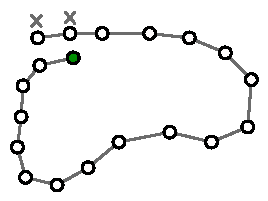
\includegraphics[width=\linewidth]{img/blob-overlap.pdf}
    \caption{A Blob with an initial overlap. To resolve, remove points
      at the end of the stroke marked with X's.}
    \label{fig:blob-overlap}
  \end{subfigure}
  \hspace{1cm} % spacing, do what you need
  \begin{subfigure}[t]{0.42\textwidth}
    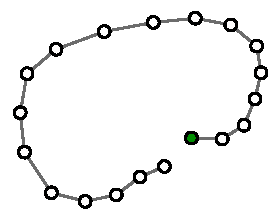
\includegraphics[width=\linewidth]{img/blob-gap.pdf}
    \caption{A Blob with an initial gap. No further action is needed.}
    \label{fig:blob-gap}
  \end{subfigure}
  \caption[Blobs: overlap vs. gap]{Two Blob shapes just before
    adjusting the start/end to match. The first is an overlap, the
    second is a gap. In case of an overlap, remove points from the end
    of the sequence until it becomes a gap. These define the initial
    spline control points.}
  \label{fig:blob}
\end{figure}


There are two possible situations: there is a \textit{gap} between the
stroke's start and end, or there is an \textit{overlap}. These cases
are illustrated in Figure~\ref{fig:blob}. The Blob Finder identifies a
gap when the first point $p_0$ is closer to the last point $p_{n-1}$
than it is to the last point's neighbors $p_{n-i}$, where i is in the
range $[2..10]$. An overlap is when $p_0$ is closer to one of the
$p_{n-i}$ points.

In case of a gap, the next action is simple: the first and last points
are connected. When an overlap is detected, the algorithm removes
points from the end of the stroke until there is no overlap
(e.g. there is a gap). Then the Blob's start and end are connected as
before.

The control points for Blob and Spline types are computed and stored
in the same manner. This representation is discussed in the Spline
section.

\subsubsection{Line Finder}

Lines are typically the most common segment type. Like arcs and
splines, lines are open segment types. A single ink stroke may contain
any number of open segment types. All open segment type finders
operate on regions between (and including) corners---they do
\textit{not} operate on the entire stroke, unless the stroke happens
to contain no corners.

The line finder fits a region of points to an idealized line, and
measure its error. If the error is below some threshold, it reports a
positive result. The idealized line begins and ends at the corners on
either side of the region. A raw point's individual error is
calculated as the shortest (orthogonal) distance between the point and
the idealized line. The total error for the region is:

\begin{equation}
Line\:Error = \dfrac{\sqrt{\sum OrthoDistance^2(p_i, line)}}{n-2}
\end{equation}

If the error is below the threshold (currently 1.5), the region is
identified as a line segment.

\subsubsection{Arc Finder}

Arcs in SIMI are portions of ellipses. If a region is not a line, the
Arc Finder attempts to identify an elliptical arc. It does this by
using the same math as Ellipse shapes, including the error metric in
Equation~\ref{eqn:ellipse}. If the total error is less than 0.5, the
region is identified as an elliptical arc.

Note that the arc is only a portion of the ellipse. The portion is
recorded using the start and end angles, and (to determine which
direction the arc traverses the ellipse) a median angle.

\subsubsection{Spline Finder}

Splines are the fallback segment type: if nothing else fits, a region
is classified as a spline. SIMI uses natural cubic splines to render
these curves.

As mentioned earlier, Blobs are modeled in the same way as
Splines. Both variations are composed of two primary points $A$ and
$B$ (for splines, the start and end points; for blobs, the start point
and initial centroid point). Using these two points, a third point $C$
is found by rotating $B$ about $A$ by 90 degrees. These three points
form the basis for a barycentric coordinate system that identify
locations of the Spline/Blob's control points. This way, when $A$ or
$B$ move, the control point locations are easily recalculated.

A control point is defined with a pair of numbers: one in the
$A\rightarrow B$ direction, another in the $A\rightarrow C$ direction. A
value of one indicates full movement from the start to end point.

\begin{figure}
  \centering
  \begin{subfigure}[t]{0.42\textwidth}
    \centering
    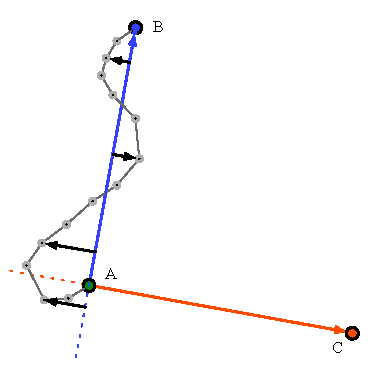
\includegraphics[width=\linewidth]{img/barycentric-spline.pdf}
    \caption{Spline primary points defined by stroke start ($A$) and
      end ($B$).}
    \label{fig:barycentric-spline}
  \end{subfigure}
  \hspace{1cm} % spacing, do what you need
  \begin{subfigure}[t]{0.42\textwidth}
    \centering
    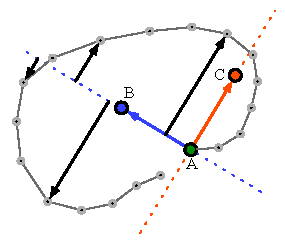
\includegraphics[width=\linewidth]{img/barycentric-blob.pdf}
    \caption{Blob primary points defined by stroke start ($A$) and
      initial centroid ($B$).}
    \label{fig:barycentric-blob}
  \end{subfigure}
  \caption[Spline and Blob Control Points]{Spline and Blob control
    points are defined in terms of two primary points, $A$ and $B$. A
    third point $C$ is simply B rotated 90 degrees about A. These
    points form the basis of a barycentric coordinate system. Control
    points are computed as a vector offset from $A$ in this coordinate
    space.}
  \label{fig:spline-blob-control-points}
\end{figure}



\section{Dynamic Recognizers}

As mentioned in \ref{sec:overview-dynamic-recognizers}, Dynamic
recognizers attempt to identify gestures as the pen is down. In order
to maintain a responsive user interface, these recognizers must
execute very quickly because they are invoked at high frequency. When
any dynamic recognizer has a positive result, the others are
suppressed until the next stroke. They each give distinct graphic
feedback to let the user know that the recognizer has triggered.

\subsection{Erase}

%% What is it for? State obvious use quickly, and give detail on any
%% non-obvious uses.

The \textit{Erase} gesture allows the user to delete segments. It lets
users recover from errors or lets them change their minds. Unlike Undo
(discussed below), Erase gives access to any linework in the
model. Erase can also be used as part of a deliberate process, for
example to cut away segments to create notches (as
in~\cite{zeleznik-lineogrammer}).

\begin{figure}
  \centering
  \begin{subfigure}[t]{0.7\textwidth}
    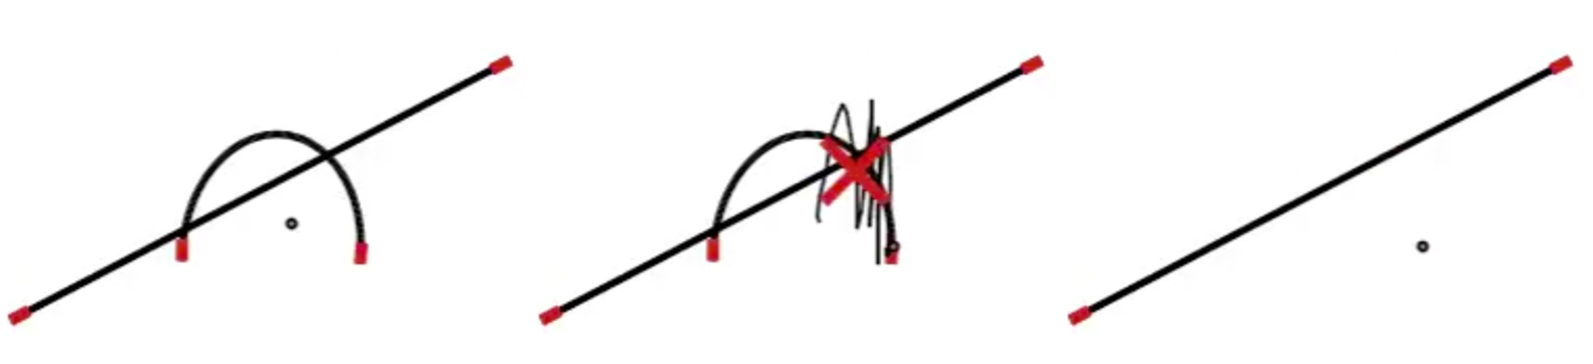
\includegraphics[width=\linewidth]{img/erase-basic.pdf}
    \caption{The erase gesture picks the most specific segments. This
      makes it easy to target short segments that are near or
      overlapping longer ones.}
    \label{fig:erase-basic}
  \end{subfigure}
  \vspace{5mm}

  \begin{subfigure}[t]{0.7\textwidth}
    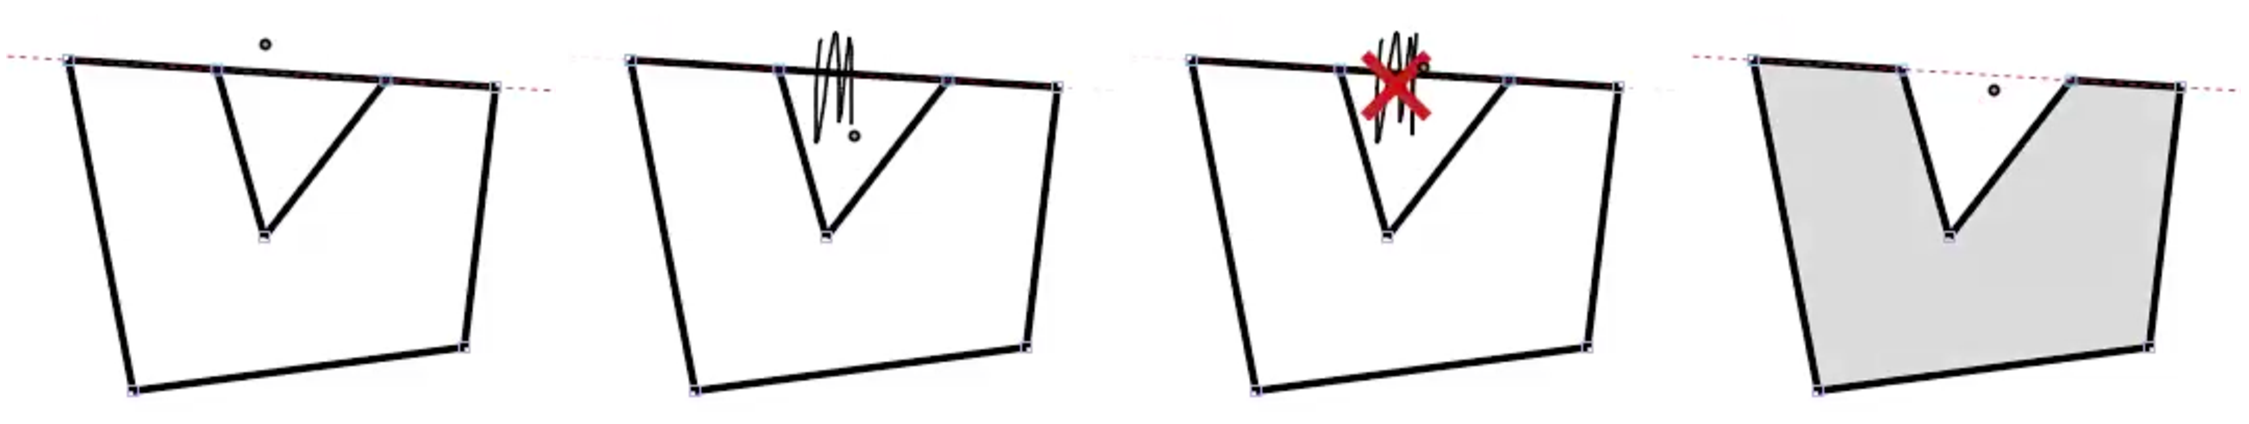
\includegraphics[width=\linewidth]{img/erase-cutout.pdf}
    \caption{Erasing can also be used as part of a deliberate process
      to subtract linework that exposes new shapes.}
    \label{fig:erase-cutout}
  \end{subfigure}
  \caption[Erase gesture]{The erase gesture is made by vigorously
    scribbling. When the dynamic recognizer identifies an erase
    gesture, it gives visual feedback (the red 'X').}
  \label{fig:erase}
\end{figure}


%% Recognition process: What kind of data does it use? What is the
%% context-free recognition like? What context does it use?

SIMI users depend on being able to erase quickly and easily. While it
may seem that an efficient and easy to use gesture recognizer would be
easy to write, this is not the case. During development, the Erase
gesture went through a number of design iterations. Initially, it was
implemented as a Delayed recognizer (executing after the pen was
lifted). Users were only able to successfully execute the gesture
about half the time. When it failed, the scribble was interpreted as
linework, requiring users to erase or undo the unwanted linework. This
was a common and frustrating event. The recognition algorithm was only
part of the problem. Proper visual feedback was also a necessary part
of the solution.

Erase was reimplemented as a dynamic recognizer so it would operate as
the pen was down. The lets it identify erase gestures in mid-stroke,
showing a colored 'X' to indicate that the user's erasure will
succeed. This gives users confidence the system has understood and
reduces the number of recognition errors substantially.

The dynamic erase gesture is implemented as follows. It involves
several parameters that may be tuned for different
circumstances. These parameters are summarized in
Table~\ref{tab:erase-params} after the description.

First we assign each point $P_i$ with a time stamp $T_i$, a
curvilinear distance $D_i$, and a heading vector $H_i$. Curvilinear
distance is the path length along the stroke from the first point:
$D_0=0$, and the rest are $D_i = D_{i-1} + distance(P_{i-1}, P_i)$.

The heading $H_i$ is a normalized vector from $P_{i-k}$ to $P_{i+k}$,
using a window size $k$. The first $k$ points use $H_k$ for their
heading.

Next we add points to a list of sample points $S$. If the curvilinear
distance between $D_i$ and the most recently added sample point is
greater than $min_{sd}$, $P_i$ is added to $S$. When a new sample
point is added, a sub-list $R$ is assembled containing recent sample
points that occurred within $t$ milliseconds. If the angle between the
new sample point's heading and any point heading in $R$ is greater
than some angle threshold value $min_\theta$ (we use $\pi$ radians),
it increments a `corner' count value for the current pen stroke. When
more than $min_c$ corners are found in a stroke, the stroke is a
strong candidate to be interpreted as an erase. When the corner count
has reached $min_c$, the system checks to see if the input resembles a
circle. This final check is necessary to avoid confusing a latch
gesture as an erase gesture. 

If the circle check fails, the stroke is interpreted as an
erasure. The system draws feedback to alert the user that the gesture
has been recognized and halts recognition until the pen is lifted.


Because the sample list depends on a relatively short duration, the
user must scribble vigorously to activate the erase gesture. Erasing
is a destructive process. Even though the user may quickly recover
from an unwanted erasure with the Undo command, they are nonetheless
disconcerting. The requirement that users scribble vigorously helps to
avoid false positives.

When the user lifts their pen, SIMI determines which (if any) segments
should be removed from the model. The simplest approach would be to
identify any segment that intersects the erase gesture's convext
hull. However, this leads to poor results because users often want to
erase items that are near other items that should be kept. If this
strategy were applied, both the line and the arc in
Figure~\ref{fig:erase-basic} would be erased.

When executing an erasure, the first step is to collect all the
segments that are under the erase gesture's convex hull. Next, SIMI
calculates the percentage of each segment's length that is under the
hull. 

It is common that users would like to erase several items with the
same gesture. To support this, SIMI chooses the segment that has the
highest percentage and any segment whose coverage is at least $C\%$ of
that value. In Figure~\ref{fig:erase-basic} about 10\% of the line is
under the hull, while about 50\% of the arc is. In the current version
of SIMI, $C=70$, so any segment that is at least 70\% of 50 (in other
words, 35\%) would be erased. Since the line is only 10\% under the
hull, it remains.

This set of segments are then removed from the model. Further, any
constraints that are no longer relevant are also removed.

% in the ``tabular'' environment, indicate columns separated by pipe
% characters. options are:
%   l           left aligned column
%   c           center aligned column
%   r           right aligned column
%   p{width}    paragraph column, text at the top
%   m{width}    ''                ''   in the middle
%   b{width}    ''                ''   at the bottom

\begin{table}%[h] % [h]ere [t]op [b]ottom [p]age
\centering
\begin{tabular}{p{1.5cm}| p{1.5cm} | p{12cm}}
\textbf{Param.} & \textbf{Value} & \textbf{Remark} 
\\ \hline
 & &
\\
$k$ &

1 &

Number of points in heading vector window. For higher resolution input
surfaces $k$ should be larger because the input points will be much
closer together.

\\

$min_{sd}$ & 

20 &

Minimum curvilinear distance between sample points. Smaller values
allow users to make smaller erase gestures, but might also introduce
false positives. 

\\

$t$ &

100ms &

Limits the sample history so only the most recent samples are
used. Samples older than this may be discarded.

\\

$min_\theta$ &

$\pi/2$ rad. &

Minimum corner angle between a recent sample heading and the current
sample heading. 

\\

$min_c$ &

5 &

Minimum number of corners required for a stroke to be an erasure.

\\

$C$ &

$70$ &

A percentage value in the range [0..100] describing how strictly to
choose erasure targets. A low value indicates few targets. Using zero
means only the most specific segment is erased; 100 means all segments
that intersect the erase gesture would be erased.

\end{tabular}
\caption{Parameters involved in detecting erase gestures.}
\label{tab:erase-params}
\end{table}


\subsection{Undo and Redo}

There is very little \textit{recognition} involved with SIMI's
\textit{Undo/Redo} recognizer. The user presses the button with their
non-dominant hand and then drags the stylus left (to undo) or right
(to redo). It is the only technique that can not be performed entirely
with the pen. While it might not require recognition like the others,
it does have to fit into the same framework.

The undo/redo events are triggered with each 40 pixel change in
the~$x$ dimension. Each event shows a preview of what the model looked
like at some point in time. Releasing the external button commits the
change by replacing the current state with the previewed state. The
user may lift the pen, reposition their hand, and continue
gesturing. This allows the user to smoothly `scrub' through their
model's design history. Each `page' in SIMI's user interface has a
separate design history.

Each state in the design history stores a complete snapshot of the
model (containing points, segments, constraints, and cutouts) as well
as a cached graphic. This is a fast memory-intensive strategy that
requires only minimal computation. Snapshots are made when the user
adds, modifies, or removes geometry or constraints.

\subsection{Flow selection}

\begin{figure}
  \centering
  \begin{subfigure}[t]{0.95\textwidth}
    \centering
    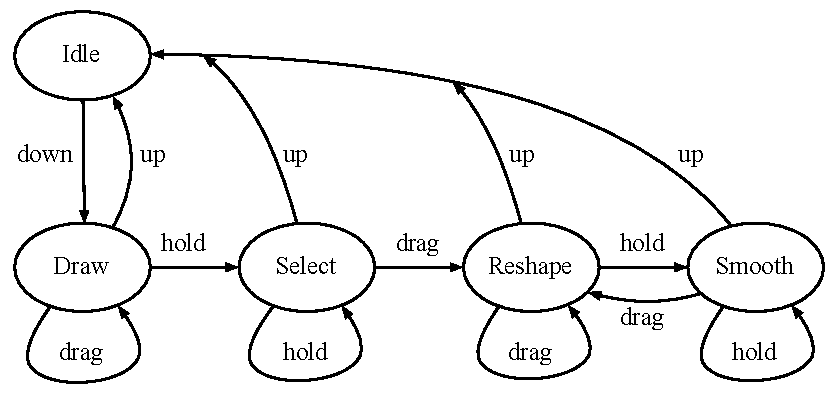
\includegraphics[width=0.5\linewidth]{img/flow-selection-fsm.pdf}
    \caption{Finite state machine that models flow
    selection. Most of the time, users simply press the pen down, draw
    some ink, and release. But if they hold the pen down, the flow
    selection states are reached. The user holds down the pen to
    select a region, moves the pen to move the selection, and holds it
    still once again to smooth the selection. Lifing the pen ends the
    process.}
    \label{fig:flow-selection-fsm}
  \end{subfigure}
  
  \vspace{5mm}
  \begin{subfigure}[t]{0.95\textwidth}
    \centering
    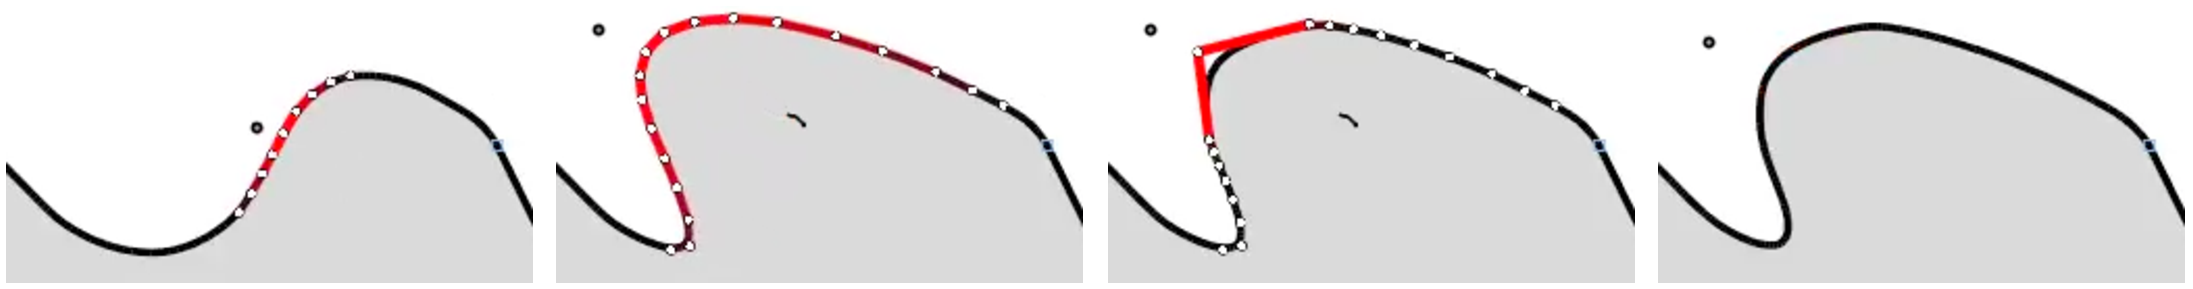
\includegraphics[width=\linewidth]{img/flow-selection-example.pdf}
    \caption{Example showing the user deforming a curved segment. The
      user holds the pen to heat a region, and moves the stylus to
      move that region. Next the user dwells to smooth region. The
      final state is at right.}
    \label{fig:flow-selection-example}
  \end{subfigure}
  \caption[Flow Selection]{Interaction and implementation of Flow Selection.}
  \label{fig:flow-selection}
\end{figure}


\textit{Flow selection} is a time-based selection and operation
technique that lets users deform \textit{regions} of curved
segments~\cite{johnson-flow-selection}. This is useful for fixing
errors, or simply playing with curves to achieve an esthetically
pleasing effect.

Flow selection is triggered by holding the pen still for a brief
period (e.g. 800 milliseconds). Once triggered, it begins selecting
points on segment nearest the stylus (see
Figure~\ref{fig:flow-selection-example}). The selection slowly grows
along the curve, as its points begins to `heat up' near the
stylus. The longer the pen is held down, the more strongly points are
selected (e.g. they become `hotter'), and the selection size gets
bigger. Next, the user can move the stylus without lifting. This moves
selected points---the more strongly selected, the more they move. The
process is nicely illustrated by the finite state machine in
Figure~\ref{fig:flow-selection-fsm}.

Flow selection is graphically presented by highlighting the affected
region. Points that have positive selection strength are drawn as
small white dots, and the linework connecting them is drawn in a shade
of red. The stronger the surrounding points, the brighter red the
curve is drawn.

\section{Pen Up Recognizers}

Introduce the pre-processing done at this point.

%% \begin{itemize}
%% \item Remove hooks
%% \item Get structured ink related to unprocessed ink.
%% \item Add all new structured ink to the model
%% \item Apply post-hoc recognizers to new structured ink
%% \item Disambiguate any conflicting results using (a) context in the
%%   model and (b) preset rules like right-angle wins over same-length
%%   (filterRecognizedItems())
%% \item Apply remaining recognized items. This removes the related
%%   structured ink from the model.
%% \item Auto-latch remaining segments with each other and existing model
%%   segments.
%% \item Search for cutouts (don't call them stencils anymore)
%% \item Wake up constraint solver
%% \item Request state snapshot
%% \end{itemize}

\subsection{Latching}

What is it for? State obvious use quickly, and give detail on any
non-obvious uses.

Recognition process: What kind of data does it use? What is the
context-free recognition like? What context does it use?

What (if any) visual feedback is there?

What actions are taken if it is positively recognized and not
filtered?

Four kinds: automatic, endpoint, continuation, and t-junction.

\subsection{Pan and Zoom}

What is it for? State obvious use quickly, and give detail on any
non-obvious uses.

Recognition process: What kind of data does it use? What is the
context-free recognition like? What context does it use?

What (if any) visual feedback is there?

What actions are taken if it is positively recognized and not
filtered?

\subsection{Select point}

What is it for? State obvious use quickly, and give detail on any
non-obvious uses.

Recognition process: What kind of data does it use? What is the
context-free recognition like? What context does it use?

What (if any) visual feedback is there?

What actions are taken if it is positively recognized and not
filtered?

\section{Delayed Recognizers}

\subsection{Same length}

What is it for? State obvious use quickly, and give detail on any
non-obvious uses.

Recognition process: What kind of data does it use? What is the
context-free recognition like? What context does it use?

What (if any) visual feedback is there?

What actions are taken if it is positively recognized and not
filtered?

\subsection{Specific length}

What is it for? State obvious use quickly, and give detail on any
non-obvious uses.

Recognition process: What kind of data does it use? What is the
context-free recognition like? What context does it use?

What (if any) visual feedback is there?

What actions are taken if it is positively recognized and not
filtered?

\subsection{Right angle}

What is it for? State obvious use quickly, and give detail on any
non-obvious uses.

Recognition process: What kind of data does it use? What is the
context-free recognition like? What context does it use?

What (if any) visual feedback is there?

What actions are taken if it is positively recognized and not
filtered?

\subsection{Same angle}

What is it for? State obvious use quickly, and give detail on any
non-obvious uses.

Recognition process: What kind of data does it use? What is the
context-free recognition like? What context does it use?

What (if any) visual feedback is there?

What actions are taken if it is positively recognized and not
filtered?
